% ThinkStack -- V Semester project report.
%
% Structure follows the department template. Every quantity in this document
% was measured against the repository or a running build; none is estimated.
% Where a number appears, the section says how it was obtained.
\documentclass[12pt,a4paper]{report}
\input{preamble}

\usepackage{titlesec}
\titleformat{\chapter}[display]
  {\normalfont\Large\bfseries}{\chaptertitlename\ \thechapter}{12pt}{\LARGE}
\titlespacing*{\chapter}{0pt}{-20pt}{24pt}

\begin{document}

% ============================================================
% COVER
% ============================================================
\thispagestyle{empty}
\begin{center}
  \vspace*{0.6cm}
  
\includegraphics[width=0.42\linewidth]{assets/christ-logo.png}\par
  \vspace{1.0cm}
  {\LARGE\bfseries ThinkStack: An Offline Small-Language-Model\\[0.3em]
   Research Assistant for Literature Review and Writing\par}
  \vspace{1.4cm}
  {\large by\par}
  \vspace{0.6cm}
  {\large Aditya Mehta (2440204)\par}
  {\large Jitvan Chadha (2440222)\par}
  {\large Ritesh K R (2440233)\par}
  \vspace{1.4cm}
  {\large Under the guidance of\par}
  % 0.6cm, matching the gap under "by" above: the two blocks are the same
  % shape and were reading as different ones at 0.4.
  \vspace{0.6cm}
  {\large\bfseries Dr. New Begin\par}
  \vspace{1.8cm}
  {\normalsize A Project report submitted in partial fulfilment of the
   requirements of\par}
  {\normalsize V Semester B.Sc. (Computer Science and Statistics)\par}
  \vspace{0.5cm}
  {\normalsize CHRIST (Deemed to be University)\par}
  \vspace{1.6cm}
  {\normalsize August 2026\par}
\end{center}
\clearpage

% ============================================================
% CERTIFICATE
% ============================================================
\thispagestyle{empty}
\begin{center}
  
\includegraphics[width=0.42\linewidth]{assets/christ-logo.png}\par
  \vspace{0.8cm}
  {\Large\bfseries CERTIFICATE}
\end{center}
\vspace{0.8cm}

This is to certify that the report titled \textbf{ThinkStack: An Offline
Small-Language-Model Research Assistant for Literature Review and Writing} is a
bona fide record of work done by \textbf{Aditya Mehta (2440204)},
\textbf{Jitvan Chadha (2440222)} and \textbf{Ritesh K R (2440233)} of CHRIST
(Deemed to be University), Bangalore, in partial fulfilment of the requirements
of V Semester B.Sc. (Computer Science and Statistics) during the year 2026--2027.

\vspace{2.0cm}
\noindent\begin{tabularx}{\linewidth}{@{}X X@{}}
\textbf{Head of the Department} & \textbf{Project Guide} \\
\end{tabularx}

\vspace{1.6cm}
\noindent\textbf{Valued-by:}

\vspace{0.5cm}
\noindent 1.\hrulefill

\vspace{0.7cm}
\noindent 2.\hrulefill

\vspace{1.4cm}
\noindent\begin{tabularx}{\linewidth}{@{}l@{\hspace{0.6em}}c@{\hspace{0.6em}}X@{}}
Examination Centre & : & CHRIST (Deemed to be University) \\[0.7em]
Date of Exam       & : & \hrulefill \\
\end{tabularx}

\clearpage

% ============================================================
% DECLARATION OF AI TOOLS
% ============================================================
\thispagestyle{empty}
\begin{center}{\Large\bfseries DECLARATION OF AI TOOL USAGE}\end{center}
\vspace{0.8cm}

We declare that the following artificial-intelligence tools were used during
the development of this project, in the roles stated.

The design of the software: its architecture, the decision to run every
inference on the user's own machine, the module boundaries, the data model and
the behaviour of each feature: is the developers' own. Claude was used to
implement the front end and to draft documentation. Every contribution it made
was reviewed before it was accepted.

\vspace{0.5cm}
\begin{longtable}{@{}p{0.24\linewidth}p{0.70\linewidth}@{}}
\toprule
\textbf{Tool} & \textbf{Role in the project} \\
\midrule
\endhead

\textbf{Claude} (Anthropic) &
Implementation of the front end, and drafting of documentation. Software
design, architecture and feature behaviour were specified by the developers;
the decision log in \texttt{docs/ADR.md} records that reasoning, and every
generated change was reviewed before it was committed. \\
\addlinespace

\textbf{Qwen2.5 0.5B / 1.5B} (Alibaba, quantised GGUF) &
Not a development tool but the \emph{product itself}. These models are bundled
with, or downloaded by, the application and perform summarisation, claim
extraction, gap analysis and \LaTeX{} generation entirely on the user's
machine. No hosted language model is used at runtime. \\
\addlinespace

\textbf{all-MiniLM-L6-v2} (Sentence-Transformers) &
The embedding model used for semantic search and for placing papers on the
literature map. It runs locally and is bundled with the application. \\
\addlinespace

\bottomrule
\end{longtable}

\vspace{1cm}
\noindent Date: 17 August 2026
\clearpage

% ============================================================
% ACKNOWLEDGEMENTS
% ============================================================
\thispagestyle{empty}
\begin{center}{\Large\bfseries ACKNOWLEDGEMENTS}\end{center}
\vspace{0.8cm}

We thank our guide, Dr. New Begin, for supervision throughout the project, and
the Department of Computer Science, CHRIST (Deemed to be University), for the
facilities and the opportunity to undertake this work.

We also thank the twelve testers who installed the pre-release builds on their
own machines. Several defects recorded in this report, including a graphics
configuration that reported no accelerator on hardware that had one, were
found only because the application was run somewhere other than the machines it
was written on.

\clearpage

% ============================================================
% ABSTRACT
% ============================================================
\thispagestyle{empty}
\begin{center}{\Large\bfseries ABSTRACT}\end{center}
\vspace{0.8cm}

A literature review requires a researcher to collect papers, read them, find
what they collectively argue, identify what they do not yet answer, and write
the result. The tools that assist with this are almost without exception hosted
services: the document is uploaded, a remote language model reads it, and the
answer is returned. That arrangement is unavailable to a researcher whose
material is unpublished, institutionally restricted or personally identifiable,
and it carries a per-query cost that a student project cannot meet.

ThinkStack performs the same work with no network. A quantised small language
model runs on the user's own processor; embeddings are computed locally; the
typesetting engine is bundled with the installer. The application ingests PDFs,
extracts their bibliographic metadata from page geometry, indexes them for
semantic search, places them on a map by meaning, identifies gaps between them,
and provides a \LaTeX{} editor that compiles offline.

The system is a desktop application built on a Python FastAPI backend, a React
interface and a Rust (Tauri) shell, distributed as signed installers for Linux,
Windows and macOS. It has been released publicly through fifteen versions.

Two results are reported. First, metadata extraction was rebuilt to read
positioned glyphs rather than flattened text, and measured against 56 papers
sampled at random across 15 arXiv subject classifications, using the archive's
own catalogue as ground truth: \textbf{92.9\% of titles and 85.7\% of author
lists exactly correct}, against a prior implementation that produced no usable
author list on any published paper tested. Second, the constraint the project
was built under, competitive quality on a consumer laptop with no network
and no accelerator, is itself the contribution, since the established tools
in this area assume a server.

\vspace{0.6cm}
\noindent\textbf{Keywords:} small language models, edge inference, offline
systems, literature review, retrieval-augmented generation, document layout
analysis, \LaTeX{}.

\clearpage

% ============================================================
% CONTENTS
% ============================================================
\pagenumbering{roman}
\setcounter{page}{1}
\tableofcontents
\clearpage
\listoftables
\clearpage
\listoffigures
\clearpage

% ============================================================
% ABBREVIATIONS
% ============================================================
\chapter*{LIST OF ABBREVIATIONS}
\addcontentsline{toc}{chapter}{List of Abbreviations}
\begin{longtable}{@{}p{0.18\linewidth}p{0.76\linewidth}@{}}
\toprule
\textbf{Abbreviation} & \textbf{Expansion} \\
\midrule
\endhead
ADR      & Architecture Decision Record \\
API      & Application Programming Interface \\
CI       & Continuous Integration \\
CPU      & Central Processing Unit \\
CRF      & Conditional Random Field \\
DFD      & Data Flow Diagram \\
DOI      & Digital Object Identifier \\
ER       & Entity--Relationship \\
GGUF     & GPT-Generated Unified Format (quantised model container) \\
GPU      & Graphics Processing Unit \\
GUI      & Graphical User Interface \\
JSON     & JavaScript Object Notation \\
LLM      & Large Language Model \\
NFC/NFKC & Unicode Normalisation Forms (Composition / Compatibility) \\
OCR      & Optical Character Recognition \\
PDF      & Portable Document Format \\
RAG      & Retrieval-Augmented Generation \\
REST     & Representational State Transfer \\
SLM      & Small Language Model \\
SRS      & Software Requirements Specification \\
TTS      & Text-to-Speech \\
UI/UX    & User Interface / User Experience \\
VRAM     & Video Random Access Memory \\
\bottomrule
\end{longtable}
\clearpage

\pagenumbering{arabic}
\setcounter{page}{1}

% ============================================================
\chapter{INTRODUCTION}
% ============================================================

\section{Project Description}

ThinkStack is a desktop research assistant that reads a collection of academic
papers and helps its user review and write about them, running entirely on the
machine it is installed on.

The user adds PDFs. Each is parsed, its bibliographic metadata extracted, its
text divided into passages, and each passage converted into a vector by an
embedding model. From that index the application provides four capabilities,
which the interface presents as four screens:

\begin{itemize}[leftmargin=*]
  \item \textbf{Library}, the collection: what has been ingested, what has
        been read, what is incomplete, and what the machine is running.
  \item \textbf{LitGraph}, the collection drawn as a map, papers placed by
        meaning rather than by folder, with themes as territories and gaps as
        markers. Search, analysis and gap-finding operate on a selection made
        on the map itself.
  \item \textbf{Scribe}, a \LaTeX{} editor with a bundled typesetting engine,
        an auto-healing compiler, and a natural-language-to-markup path that is
        grounded on the user's own papers.
  \item \textbf{Bench}: what the machine can run, which model serves which
        task, and how to add or remove models.
\end{itemize}

Every inference is local. The single optional network request is a version
check against the releases page, which transmits no user data and fails
silently when offline.

\section{Existing System}

Tools that assist with literature review fall into three groups, and each is
unusable under at least one of this project's constraints.

\subsection{Hosted research assistants}

Elicit, SciSpace, Consensus and comparable services upload the document and
answer from a remote large language model. They are capable and, for a large
class of users, the correct choice. They are unavailable to a researcher whose
material cannot leave the machine: unpublished results, institutionally
restricted corpora, or documents containing personal data, and they charge
per query, which a student project cannot sustain.

\subsection{Reference managers}

Zotero and Mendeley manage citations well and do not read the papers. They
organise; they do not answer questions about content, find gaps, or write.

\subsection{Hosted \LaTeX{} editors}

Overleaf compiles in the cloud, which introduces a queue, a time limit and a
network dependency, and requires an account. It also has no knowledge of the
user's library, so a citation must be fetched by hand from elsewhere.

\subsection{What none of them do}

None runs the model on the user's own machine. The gap ThinkStack addresses is
not a missing feature in any one of these tools; it is that the entire category
assumes a server, and therefore assumes the document may be sent to one.

\section{Objectives}

\begin{enumerate}[leftmargin=*]
  \item Run every inference, embedding, summarisation, claim extraction, gap
        analysis and text generation, on the user's own hardware, with no
        hosted language model at any point.
  \item Remain fully functional with no network connection.
  \item Extract bibliographic metadata accurately enough that it can label a
        paper elsewhere in the application and populate a citation.
  \item Represent a collection as a structure rather than a list, so that the
        relationships between papers and the gaps between them are visible.
  \item Compile \LaTeX{} locally, with a bundled engine, so that writing has no
        queue, no account and no time limit.
  \item Size the workload to the machine, so that the application is usable on
        a consumer laptop rather than requiring an accelerator.
  \item Distribute as installers for Linux, Windows and macOS, verified by
        running the packaged application rather than by a green build.
\end{enumerate}

\section{Purpose, Scope and Applicability}

\subsection{Purpose}

To make the assistance that hosted research tools provide available to
researchers who cannot use them, by moving the computation to the user's device
rather than the user's documents to a provider's.

\subsection{Scope}

The system covers ingestion of text-bearing PDFs, metadata extraction, semantic
search, summarisation, claim extraction, thematic clustering, gap analysis, a
literature map, at-rest encryption of stored documents, local \LaTeX{}
compilation, and model management including acquisition from Hugging Face.

It does not cover scanned documents with no text layer, which require OCR that
the application does not ship; collaborative editing; or synchronisation
between devices, which would contradict the premise.

\subsection{Applicability}

The system applies wherever a literature review must be conducted on material
that cannot be uploaded, or where per-query cost or network availability rules
out a hosted tool: postgraduate and doctoral research, institutions with data
governance requirements, and students without a budget for inference.

\section{Overview of the Report}

Chapter~2 states the problem formally and specifies the functional and
non-functional requirements, the system requirements, and the conceptual
models. Chapter~3 presents the architecture, the module decomposition, the
data design and the interface design. Chapter~4 describes the implementation,
the coding standards adopted, and the parts of the system whose implementation
is worth recording in detail. Chapter~5 reports the testing strategy, the test
cases and their results. Chapter~6 concludes with the design and implementation
issues encountered, the advantages and limitations of the result, and the
future scope of the work.

% ============================================================
\chapter{SYSTEM ANALYSIS}
% ============================================================

\section{Problem Definition}

Given a collection of research papers held locally, the system must let a
researcher answer four questions without any document leaving the machine:

\begin{enumerate}[leftmargin=*]
  \item \textbf{What do I have?}: identify each paper accurately enough to
        name it, and report what the application has read of it.
  \item \textbf{What does it say about $X$?}: retrieve the passages that
        answer a question posed in natural language.
  \item \textbf{What does the collection not answer?}: identify claims that
        are asserted but unsupported, and questions the corpus raises but does
        not address.
  \item \textbf{How do I write it up?}: compose and typeset the result,
        citing the collection.
\end{enumerate}

Each is constrained by the hardware the work must run on. A consumer laptop
with 8--16\,GB of memory and no usable accelerator is the target, not the
degraded case.

\section{Requirements Specification}

\subsection{Functional Requirements}

\begin{longtable}{@{}p{0.10\linewidth}p{0.34\linewidth}p{0.48\linewidth}@{}}
\caption{Functional requirements}\label{tab:fr}\\
\toprule
\textbf{ID} & \textbf{Requirement} & \textbf{Description} \\
\midrule
\endfirsthead
\toprule
\textbf{ID} & \textbf{Requirement} & \textbf{Description} \\
\midrule
\endhead

FR-1  & Ingest a PDF & Accept one or many PDFs by drag-and-drop or file
        picker; extract text; report failure per file. \\
FR-2  & Extract metadata & Determine title, authors, year and abstract from the
        document, without a network lookup. \\
FR-3  & Correct metadata & Allow a wrong title, author list or year to be
        corrected in place, and propagate the correction to every stored
        passage. \\
FR-4  & Chunk and embed & Divide text into passages and compute an embedding
        for each, locally. \\
FR-5  & Semantic search & Return ranked passages for a natural-language query,
        grouped by paper. \\
FR-6  & Summarise & Produce a summary of one or more selected papers. \\
FR-7  & Extract claims & Produce the assertions a paper makes, as structured
        output. \\
FR-8  & Cluster themes & Group the collection into themes derived from the
        embeddings. \\
FR-9  & Find gaps & Identify unsupported claims and unaddressed questions
        across a selection, and retain past runs. \\
FR-10 & Draw the map & Place papers in two dimensions by semantic similarity;
        show themes as regions and gaps as markers. \\
FR-11 & Read a paper & Display the original PDF with matched passages marked. \\
FR-12 & Encrypt at rest & Encrypt a stored document under a user password and
        decrypt on demand. \\
FR-13 & Edit and compile & Provide a \LaTeX{} editor and compile to PDF
        locally, recovering from common errors. \\
FR-14 & Manage project files & Treat a paper as a directory; support upload,
        rename, move, copy and delete within it. \\
FR-15 & Generate markup & Convert a natural-language instruction into \LaTeX{},
        optionally grounded on selected papers. \\
FR-16 & Manage models & List, import, assign, download and remove models;
        route each task to a model. \\
FR-17 & Report capability & Report what the machine can run, measured rather
        than assumed. \\
FR-18 & Update in place & Check for a new version and install it on request. \\
FR-19 & Report progress & Show what background analysis is doing and how far
        through it is. \\
FR-20 & Stop ingestion & Interrupt a running batch without leaving a document
        partly ingested. \\
FR-21 & Cite a paper & Insert a citation to a paper in the library from within
        the editor, and maintain the project's bibliography file. \\
FR-22 & Resolve citations & Compile citations to numbered references and
        generate the reference list, without the author declaring a
        bibliography. \\
\bottomrule
\end{longtable}

\subsection{Non-Functional Requirements}

\begin{longtable}{@{}p{0.10\linewidth}p{0.26\linewidth}p{0.56\linewidth}@{}}
\caption{Non-functional requirements}\label{tab:nfr}\\
\toprule
\textbf{ID} & \textbf{Attribute} & \textbf{Requirement} \\
\midrule
\endfirsthead
\toprule
\textbf{ID} & \textbf{Attribute} & \textbf{Requirement} \\
\midrule
\endhead

NFR-1 & Privacy & No document, prompt or embedding is transmitted. The only
        outbound request is a version check carrying no user data. \\
NFR-2 & Offline operation & Every feature except the update check functions
        with no network. \\
NFR-3 & Memory & The model is sized against \emph{available} memory, not
        installed memory, so the process is not terminated mid-analysis. \\
NFR-4 & Responsiveness & Ingestion returns before analysis completes; the
        interface reports the queue rather than blocking. \\
NFR-5 & Portability & One codebase produces installers for Linux, Windows and
        macOS. \\
NFR-6 & Recoverability & A malformed figure or a missing package must not cost
        the author the compiled document. \\
NFR-7 & Integrity & Encryption is authenticated, so tampering is detected at
        decryption rather than producing plausible but corrupted output. \\
NFR-8 & Maintainability & Every architectural decision is recorded with its
        reasoning; dependencies are pinned exactly. \\
NFR-9 & Verifiability & A release is validated by running the packaged
        application, not by a passing build. \\
NFR-10 & Accessibility & Text meets contrast requirements against its
        substrate; controls are reachable by keyboard. \\
\bottomrule
\end{longtable}

\section{Block Diagram}

\begin{figure}[H]
\centering
\begin{tikzpicture}[
  node distance=0.8cm,
  box/.style={draw, rounded corners=2pt, minimum width=3.1cm,
              minimum height=0.85cm, align=center, font=\small},
  lay/.style={draw, dashed, rounded corners=3pt, inner sep=0.30cm},
  ->/.default=stealth]

\node[box] (ui) {Interface (React)\\ Library · LitGraph · Scribe · Bench};
\node[box, below=of ui] (api) {REST API (FastAPI)};
\node[box, below=of api, minimum width=3.1cm] (dom) {Domain\\ ingestion ·
      analysis · search · paper writer};
\node[box, below=of dom] (inf) {Infrastructure\\ inference · vector store ·
      capability · files};
\node[box, below=of inf] (hw)  {The user's machine\\ CPU · memory · disk};

\draw[->] (ui) -- (api);
\draw[->] (api) -- (dom);
\draw[->] (dom) -- (inf);
\draw[->] (inf) -- (hw);

\node[right=1.4cm of api, box, fill=black!4] (shell) {Desktop shell\\ (Tauri /
      Rust)};
\draw[->, dashed] (shell) -- (api);
\draw[->, dashed] (shell.north) -- ++(0,0.75) -| (ui.east);
\end{tikzpicture}
\caption{Block diagram. The shell supervises the backend process and hosts the
interface; every arrow is a local call.}
\label{fig:block}
\end{figure}

\section{System Requirements}

\subsection{User Characteristics}

The intended user is a researcher, postgraduate student or academic who reads
and writes papers. Familiarity with \LaTeX{} is assumed for Scribe but not for
the rest of the application. No knowledge of language models, embeddings or
model quantisation is assumed, which is why Bench reports what the machine can
run in plain terms and the application ships with a working model rather than
asking the user to choose one.

\subsection{Software and Hardware Requirements}

\begin{longtable}{@{}p{0.28\linewidth}p{0.30\linewidth}p{0.34\linewidth}@{}}
\caption{Hardware and software requirements}\label{tab:sysreq}\\
\toprule
 & \textbf{Minimum} & \textbf{Recommended} \\
\midrule
\endfirsthead
\toprule
 & \textbf{Minimum} & \textbf{Recommended} \\
\midrule
\endhead

Operating system & Windows 10, macOS 12, or a Linux distribution with GTK/WebKit
 & Any of the above, current \\
Processor & 64-bit dual core & Quad core or better \\
Memory & 8\,GB & 16\,GB \\
Disk & 2\,GB free & 5\,GB free \\
Accelerator & None required & Vulkan-capable GPU, optional \\
Network & Not required & Required only to download an additional model \\
\bottomrule
\end{longtable}

The development and evaluation machine was a 16\,GB laptop with no usable
accelerator, running Fedora. Every figure reported in Chapter~5 was measured on
it.

\subsection{Constraints}

\begin{itemize}[leftmargin=*]
  \item \textbf{No hosted inference.} This forecloses the largest models and
        is the constraint from which most of the design follows.
  \item \textbf{Installer size.} A single release asset must remain under
        GitHub's 2\,GiB limit, which is why one small model is bundled and a
        larger one is fetched on consent.
  \item \textbf{A shared, serialised model.} One model is resident at a time,
        so concurrent analyses queue rather than compete for memory.
  \item \textbf{No OCR.} A scanned PDF with no text layer yields nothing, and
        no later stage can recover from that.
\end{itemize}

\section{Conceptual Models}

\subsection{Data Flow Diagram}

\begin{figure}[H]
\centering
\begin{tikzpicture}[
  node distance=1.05cm and 1.5cm,
  proc/.style={draw, rounded corners=8pt, minimum width=2.5cm,
               minimum height=0.8cm, align=center, font=\small},
  store/.style={draw, minimum width=2.5cm, minimum height=0.7cm,
                align=center, font=\small, fill=black!4},
  ext/.style={draw, minimum width=2.0cm, minimum height=0.7cm,
              align=center, font=\small}]

\node[ext]   (user)  {Researcher};
\node[proc, right=of user] (ing) {1.0\\Ingest};
\node[store, right=of ing] (vs) {Vector store};
\node[proc, below=of ing] (ana) {2.0\\Analyse};
\node[store, right=of ana] (cache) {Analysis cache};
\node[proc, below=of ana] (wri) {3.0\\Write};
\node[store, right=of wri] (proj) {Project files};

\draw[->] (user) -- node[above, font=\tiny] {PDF} (ing);
\draw[->] (ing)  -- node[above, font=\tiny] {passages} (vs);
\draw[->] (vs)   -- node[right, font=\tiny] {embeddings} (cache);
\draw[->] (ing)  -- node[right, font=\tiny] {text} (ana);
\draw[->] (ana)  -- node[above, font=\tiny] {summaries, gaps} (cache);
\draw[->] (ana)  -- node[right, font=\tiny] {grounding} (wri);
\draw[->] (wri)  -- node[above, font=\tiny] {.tex, .pdf} (proj);
\draw[->] (user.south) |- node[below, font=\tiny, pos=0.25] {query, instruction} (wri.west);
\end{tikzpicture}
\caption{Level-1 data flow. No process crosses the machine boundary.}
\label{fig:dfd}
\end{figure}

\subsection{Entity--Relationship Diagram}

\begin{figure}[H]
\centering
\begin{tikzpicture}[
  ent/.style={draw, minimum width=2.6cm, minimum height=0.8cm,
              align=center, font=\small},
  rel/.style={draw, diamond, aspect=2, align=center, font=\tiny,
              inner sep=1pt}]

\node[ent] (doc)   {Document};
\node[rel, right=1.2cm of doc] (has) {divided into};
\node[ent, right=1.2cm of has] (chunk) {Chunk};
\node[ent, below=1.5cm of doc] (run) {Analysis run};
\node[rel, right=1.2cm of run] (cov) {covers};
\node[ent, below=1.5cm of chunk] (gap) {Gap};
\node[ent, below=1.5cm of run] (proj) {Paper project};

\draw (doc) -- node[above, font=\tiny] {1} (has);
\draw (has) -- node[above, font=\tiny] {N} (chunk);
\draw (run) -- node[above, font=\tiny] {1} (cov);
\draw (cov) -- node[above, font=\tiny] {N} (gap);
\draw (doc) -- node[left, font=\tiny] {N} (run);
\draw (run) -- (proj);
\end{tikzpicture}
\caption{Entities and their relationships. A document owns its chunks; an
analysis run covers a selection of documents and produces gaps.}
\label{fig:er}
\end{figure}

% ============================================================
\chapter{SYSTEM DESIGN}
% ============================================================

\section{System Architecture}

The application is four layers and a shell, and the direction of dependency is
strictly downward: the interface knows the API, the API knows the domain, the
domain knows infrastructure, and nothing knows the layer above it.

\begin{longtable}{@{}p{0.22\linewidth}p{0.74\linewidth}@{}}
\caption{Architectural layers}\label{tab:layers}\\
\toprule
\textbf{Layer} & \textbf{Responsibility} \\
\midrule
\endfirsthead
\toprule
\textbf{Layer} & \textbf{Responsibility} \\
\midrule
\endhead

\texttt{frontend/} & The interface. React~19 and Vite, one theme, four screens.
  Holds no business rule: anything derived from global state is read from the
  backend rather than recomputed. \\
\addlinespace
\texttt{api/} & REST endpoints. Validates, orchestrates, and returns; contains
  no domain logic of its own. \\
\addlinespace
\texttt{domain/} & The capabilities, one package each: \texttt{ingestion},
  \texttt{knowledge\_base}, \texttt{search}, \texttt{analysis},
  \texttt{litgraph}, \texttt{paper\_writer}, \texttt{model\_manager}. Pure
  Python, no framework imports. \\
\addlinespace
\texttt{infrastructure/} & Everything that touches the machine: the inference
  client, the vector store, the capability model, file management, the job
  queue, encryption. \\
\addlinespace
\texttt{src-tauri/} & The desktop shell, in Rust. Starts the backend as a
  supervised child process, waits behind a loading screen, and stops it when
  the window closes. \\
\bottomrule
\end{longtable}

\evidence{\textbf{Decision recorded.} One module answers ``what can this machine
do''. Before \texttt{infrastructure/capability.py} existed, that question was
answered in about ten places and two of them disagreed, the Rust diagnosis
chose GPU layers and a Python module computed them again, with the Rust answer
winning at runtime. The Python one was therefore unreachable code that still
looked authoritative. The split is now: \emph{Rust detects, Python decides.}}

\section{Module Design}

\begin{longtable}{@{}p{0.26\linewidth}p{0.70\linewidth}@{}}
\caption{Module decomposition}\label{tab:modules}\\
\toprule
\textbf{Module} & \textbf{Contents} \\
\midrule
\endfirsthead
\toprule
\textbf{Module} & \textbf{Contents} \\
\midrule
\endhead

\texttt{ingestion} & \texttt{pdf\_parser} (text and positioned spans),
  \texttt{layout} (geometry: rows, cells, normalisation), \texttt{layout\_metadata}
  (title and authors from geometry), \texttt{metadata\_extractor}
  (orchestration and fallbacks), \texttt{chunker}. \\
\addlinespace
\texttt{knowledge\_base} & \texttt{embedding\_service}, \texttt{repository}
  (storage and retrieval of chunks with their metadata). \\
\addlinespace
\texttt{search} & Semantic search over chunk embeddings, with optional
  grouping by document. \\
\addlinespace
\texttt{analysis} & \texttt{summarizer}, \texttt{claim\_extractor},
  \texttt{theme\_clusterer}, \texttt{precompute} (queues work at ingest so the
  canvas is ready before it is opened). \\
\addlinespace
\texttt{litgraph} & \texttt{graph\_builder}: positions, themes and gap markers
  derived on request from embeddings and past runs. \\
\addlinespace
\texttt{paper\_writer} & \texttt{compiler} (Tectonic or pdflatex, with error
  recovery), \texttt{files} (a project is a directory, with a path boundary),
  \texttt{indexing}. \\
\addlinespace
\texttt{model\_manager} & \texttt{registry}, \texttt{catalog},
  \texttt{router}, \texttt{downloader}, \texttt{manifest}. \\
\bottomrule
\end{longtable}

\section{Database Design}

\subsection{Tables and Relationships}

The system stores five things, all under the user's data directory. There is no
relational database: the store is a vector index with per-record metadata, plus
JSON documents and directories on disk. That is a deliberate choice, a
relational engine would add an installed dependency to an application whose
premise is that it runs on a laptop with nothing configured, and the
consequence is that referential integrity is enforced in the repository layer
rather than by a foreign key.

\begin{longtable}{@{}p{0.24\linewidth}p{0.30\linewidth}p{0.42\linewidth}@{}}
\caption{Persistent stores}\label{tab:stores}\\
\toprule
\textbf{Store} & \textbf{Form} & \textbf{Contents} \\
\midrule
\endfirsthead
\toprule
\textbf{Store} & \textbf{Form} & \textbf{Contents} \\
\midrule
\endhead

Vector store & Embedded chunks & \texttt{chunk\_id}, \texttt{doc\_id},
  \texttt{text}, \texttt{embedding}, \texttt{page\_number},
  \texttt{chunk\_index}, \texttt{token\_count}, and the paper's
  \texttt{title}, \texttt{authors}, \texttt{year}. \\
\addlinespace
Papers directory & Original PDFs & The uploaded file, unmodified, addressed by
  \texttt{doc\_id}. \\
\addlinespace
Analysis cache & JSON & Per document: summary and extracted claims. \\
\addlinespace
Run histories & JSON & Analysis and gap runs, newest first, capped. \\
\addlinespace
Paper projects & Directories & One directory per paper, containing
  \texttt{main.tex}, figures and build artefacts. \\
\bottomrule
\end{longtable}

\subsection{Data Integrity and Constraints}

\begin{itemize}[leftmargin=*]
  \item Bibliographic metadata is duplicated onto every chunk so that a search
        result can name its paper without a second lookup. The cost is that
        correcting a title is not one write but a write to every chunk of the
        document; missing one would let the same paper answer to two titles
        depending on which passage matched.
  \item Deleting a document deletes its chunks, its stored PDF and its cached
        analysis together.
  \item Encryption is applied to chunk text in the store. The original PDF is
        \emph{not} encrypted, so the route that serves it refuses to do so for
        an encrypted document: serving it would hand back exactly what the
        encryption exists to withhold.
  \item A gap run supersedes the one before it: the newest run is the library's
        current state, not the sum of all runs.
\end{itemize}

\section{System Configuration}

Configuration is derived rather than declared wherever possible. The capability
model measures the machine at startup and every downstream number: context
size, GPU layers, output token budget, how much of a paper fits in one prompt
is computed from that measurement rather than set in a file. Dependencies
are pinned exactly, and a check in CI fails the build if a range appears, since
a range lets the same commit build a different program tomorrow.

\section{Interface Design and Procedural Design}

\subsection{User Interface Design}

The interface is one theme, described internally as \emph{Paper and Ink}: a
sheet of paper on a desk, worked in ink. Four surfaces, one ink ramp of four
steps, a single 2\,px radius and two shadows. Type is a six-step scale on a
fluid root, so every measurement grows with the window rather than sitting at a
fixed size on a large display.

Three principles govern it, and each was arrived at by correcting its opposite:

\begin{enumerate}[leftmargin=*]
  \item \textbf{The interface reads the backend's answer; it never recomputes
        it.} A panel that decided for itself which model was in use displayed
        the wrong one for every release in which it existed.
  \item \textbf{A figure earns its place by answering a question the reader
        would ask.} Counts that described the implementation, bytes on disk,
        the number of index fragments, were removed rather than restyled.
  \item \textbf{Nothing is withheld.} A collapsed navigation panel keeps a rail
        rather than disappearing, because at zero width the controls it still
        owed the reader had to be drawn on top of the page.
\end{enumerate}

\subsection{Application Flow and Class Diagram}

Figure~\ref{fig:flow} traces one paper from the moment it is dropped on the
window to the moment it can be cited, which is the path that crosses every
module in the system.

\begin{figure}[H]
\centering
\begin{tikzpicture}[
  node distance=0.55cm,
  step/.style={draw, rounded corners=2pt, minimum width=8.2cm,
               minimum height=0.62cm, align=left, font=\small,
               inner xsep=6pt},
  ->=stealth]
\node[step] (a) {1. \textbf{UploadPanel}: file accepted, queued};
\node[step, below=of a] (b) {2. \textbf{pdf\_parser}: text, and spans with size and baseline};
\node[step, below=of b] (c) {3. \textbf{layout}: spans grouped into rows, rows into cells};
\node[step, below=of c] (d) {4. \textbf{layout\_metadata}: title and authors by named rules};
\node[step, below=of d] (e) {5. \textbf{metadata\_extractor}: plausible? else the model};
\node[step, below=of e] (f) {6. \textbf{chunker}: passages sized for retrieval};
\node[step, below=of f] (g) {7. \textbf{embedding\_service}, a vector per passage};
\node[step, below=of g] (h) {8. \textbf{repository}: stored with its metadata};
\node[step, below=of h] (i) {9. \textbf{precompute}: summary, claims, themes, gaps queued};
\node[step, below=of i] (j) {10. \textbf{graph\_builder}, the map, derived on request};
\foreach \x/\y in {a/b,b/c,c/d,d/e,e/f,f/g,g/h,h/i,i/j} \draw[->] (\x) -- (\y);
\end{tikzpicture}
\caption{Application flow: one paper, from drop to citable.}
\label{fig:flow}
\end{figure}

Steps 1--8 complete before the upload request returns. Step 9 is deliberately
\emph{not} awaited: it costs tens of seconds per paper, and awaiting it once put
a fifty-second model call inside an HTTP request, so uploading three papers
appeared to hang the application for three minutes. The work still happens at
ingest time, so the map is ready before it is opened, it simply happens
after the response, with the queue reported in the interface.

\begin{figure}[H]
\centering
\begin{tikzpicture}[
  cls/.style={draw, minimum width=3.5cm, align=center, font=\small,
              inner sep=4pt},
  ->=stealth]
\node[cls] (meta) {\textbf{DocumentMetadata}\\[2pt]
  \footnotesize title, authors, abstract,\\ \footnotesize year, source, pages};
\node[cls, right=1.6cm of meta] (doc) {\textbf{Document}\\[2pt]
  \footnotesize doc\_id, filename, path,\\ \footnotesize metadata, chunks, status};
\node[cls, below=1.2cm of doc] (chunk) {\textbf{TextChunk}\\[2pt]
  \footnotesize chunk\_id, doc\_id, text,\\ \footnotesize page, index, tokens};
\node[cls, below=1.2cm of meta] (span) {\textbf{TextSpan / PageLayout}\\[2pt]
  \footnotesize text, size, bbox,\\ \footnotesize baseline, horizontal};
\draw[->] (meta) -- node[above, font=\tiny] {1} (doc);
\draw[->] (doc) -- node[right, font=\tiny] {1..N} (chunk);
\draw[->] (span) -- node[below, font=\tiny] {read by} (chunk);
\draw[->] (span) -- node[left, font=\tiny] {produces} (meta);
\end{tikzpicture}
\caption{The ingestion data model. \texttt{TextSpan} carries the baseline,
which is what makes a small-capitals title recoverable.}
\label{fig:class}
\end{figure}

\section{Reports Design}

The application produces three outputs a user keeps: the compiled PDF from
Scribe; the gap-analysis run, retained in history and reopenable; and the
literature map, which is regenerated from the current index on every visit
rather than stored, so there is no stale graph to invalidate.

% ============================================================
\chapter{IMPLEMENTATION}
% ============================================================

\section{Implementation Approaches}

Three approaches shaped the implementation and are worth stating because each
replaced a plausible alternative.

\subsection{Measure, then move}

Work was moved between languages only for a measured reason. Startup diagnosis
was rewritten in Rust because the Python implementation imported a deep-learning
framework purely to discover whether a GPU existed, costing seconds on every
launch. Model discovery was measured at approximately 9\,ms and left in Python,
because the same argument does not apply to code that is already fast.

The same rule prevented a larger mistake. When metadata extraction was found to
be wrong, rewriting the pipeline in a systems language was considered. Profiling
one paper gave: extraction 6.0\,ms, metadata 1.1\,ms, chunking 0.2\,ms,
embedding and search 3073.8\,ms. Everything a rewrite would have touched was
0.3\% of runtime, and the remainder was already compiled native code. The defect
was the question being asked, not the language asking it.

\subsection{Repair rather than refuse}

A small language model produces markup that is frequently almost correct. The
compiler therefore inserts missing package declarations, wraps bare fragments
into complete documents, and progressively neutralises a failing environment
and retries, so one malformed figure does not cost the author the document.

\subsection{Record the reasoning, not the change}

Every architectural decision is recorded in \texttt{docs/ADR.md} with its
context and its consequences. The log reached 40 entries. Its value was not
apparent while it was being written and became apparent during the dependency
audit, when the reasoning behind earlier choices could be read rather than
reconstructed.

\section{Coding Standard}

\begin{itemize}[leftmargin=*]
  \item \textbf{Python}: \texttt{ruff} in CI, no warnings tolerated;
        type hints on module boundaries; no framework imports inside
        \texttt{domain/}.
  \item \textbf{JavaScript}: ESLint with the React hooks rules; zero errors
        required to merge. The hooks linter caught a genuine defect during this
        work: a ref read during render.
  \item \textbf{Comments}, a comment states the constraint a maintainer must
        not break, not what the line does. Rationale belongs in the decision
        log. A prose-reduction pass took comment and docstring density from
        32\% to 27\% of source lines, deleting restatements of type hints and
        of decisions recorded elsewhere.
  \item \textbf{Commits}, the reasoning goes in the commit message, and the
        history is treated as part of the deliverable.
  \item \textbf{Branching}: \texttt{main} (released), \texttt{beta}
        (testers), \texttt{dev} (integration), and short-lived
        \texttt{feat/}\,/\,\texttt{fix/} branches. Nothing reaches
        \texttt{main} without passing through the other two.
\end{itemize}

\section{Key Implementations}

\subsection{Metadata extraction from page geometry}

This is the implementation the project is most defined by, and it is the one
that was rebuilt.

The original implementation read the document as a flat string and applied
regular expressions: the title was any of the first ten lines longer than ten
characters; an author was any line beginning with two capitalised words; the
year was the first four-digit number. Measured against published papers with
known metadata, it produced no usable author list on any of them. On
\emph{Attention Is All You Need} it returned the publisher's copyright notice as
the title, listed the paper's own title and its authors' employers as authors,
and reported the year as 2014: three years before the paper existed.

The cause is that a PDF is not text. It is positioned glyphs, each carrying a
size, a bounding box and a writing direction, and \texttt{extract\_text()}
discards all of it. Typesetting convention places the title in the largest
horizontal text at the top of page~1, with the authors on the rows beneath,
a signal that is present in the file and thrown away before extraction begins.

The rebuilt implementation is two modules. \texttt{layout.py} knows about
typesetting and nothing about papers: it groups glyphs into rows and divides
each row into cells. \texttt{layout\_metadata.py} decides what a title or an
author is, as a set of named rules.

Splitting rows into cells is the single highest-value step. The PDF library
reports a four-column author row as one line, so read as text
``Kaiming He Xiangyu Zhang Shaoqing Ren Jian Sun'' is an eight-word phrase and
no filter can recover four names from it. Read as positions it is four cells.
Ablated, that one rule is worth 7 of 7 papers against 1 of 7.

Three further findings were geometric rather than bibliographic:

\begin{itemize}[leftmargin=*]
  \item Rows must be grouped by \emph{baseline}, not by bounding-box top. A
        small-capitals title is one line set in two sizes; grouped by the top,
        \emph{ADAM, A Method for Stochastic Optimization} extracted as
        ``A, A M S O''.
  \item A font change mid-word produces two spans with no gap between them.
        Inserting a space there yields ``A DAM''.
  \item \TeX{} emits an accent as a separate glyph \emph{before} its letter, so
        ``Doll\'ar'' arrives as three pieces and prints as ``Doll \'ar'',
        leaving the surname unsearchable.
\end{itemize}

Affiliations are removed without naming employers, which would be an endless and
dating list. Three rules do it instead: a structural word (\emph{university},
\emph{institute}, \emph{research}) disqualifies an entire row; a short
all-capitals token beside ordinary words is an acronym; and a phrase printed
more than once in the author region is an address, because a shared affiliation
is printed once per author while a name is printed once per paper. The third
requires no vocabulary at all and is the only rule that can separate ``United
Kingdom'' from ``Kaiming He'', which are indistinguishable by spelling.

\subsection{Sizing the work to the machine}

\texttt{capability.py} answers what the machine can do, and every derived
number comes from it. Two defects were fixed by centralising it:

\begin{itemize}[leftmargin=*]
  \item \textbf{Summarisation could not fit in its own context window.} 6000
        characters of paper plus a 1024-token reply needs roughly 2650 tokens;
        a low-capability machine is given 2048. The request failed before the
        model was asked to think, and the error handler then told the reader the
        response ``could not be read'', which was untrue.
  \item \textbf{Every Apple Silicon machine was pinned to the CPU.} GPU layers
        were decided by \texttt{has\_cuda \&\& vram\_gb >= 2.0}; Apple Silicon
        reports neither.
\end{itemize}

\subsection{The guard that tested for silence}\label{sub:silence}

A recurring defect class is worth recording as an implementation lesson. Three
separate failures had the same shape: \emph{a check that tests for silence,
when the failure mode is confident wrongness}.

A small-language-model fallback existed for papers the regular expressions could
not handle, guarded on the extracted title being \emph{empty}. The regular
expressions never returned empty, they returned wrong, so the guard never
fired on a single paper it existed to rescue. Similarly, graphics advice was
gated on a VRAM figure that only one vendor's tool reports, so machines with a
working accelerator were told they had none; and a release marked
\texttt{draft: false} was published as a draft, with every job reporting green.

The correction in each case is the same: test for the shape of a right answer,
not for the absence of one.

\subsection{A project is a directory}

Compilation always ran with the project directory as its working directory, so
relative paths in \verb|\includegraphics| resolved correctly, but there was
no way to put a second file into that directory, so a figure could be referenced
and never supplied. Exposing the directory required a path boundary: this API is
reachable from the webview, which the shell treats as remote content, so a
filename arriving at it is untrusted input. Every operation resolves its
argument against the project directory and refuses anything landing outside.
Resolution happens \emph{before} the check rather than a string test for
\texttt{..}, because that is what catches a symbolic link.

\subsection{Citations, and where the authority for a key lives}

The editor could compile a document but could not cite one. The interaction
chosen puts the library where the author already is: typing the word
\texttt{cite} opens a list beneath the cursor, further typing filters it on
title, author, year or key, and Enter replaces the word with a citation
command while writing the corresponding entry into the project's bibliography
file. Selecting nothing leaves the word in place, and an ordinary word
compiles.

Citation numbers are not tracked, and the omission is deliberate. BibTeX
renumbers every citation on each recompile and orders the reference list
according to the chosen style, so emitting keys obtains that behaviour for
nothing, whereas tracking numbers would maintain a second and less reliable
copy of it.

The design question that remained was which side holds the authority for a key.
Keys are derived from metadata, so a collision between two papers is resolved
differently depending on what else the library contains, and a key derived
again later can differ from the one already written into the author's source.
The bibliography file is therefore authoritative: keys already present in it are
honoured and never recomputed, and only documents the file has not seen are
assigned new ones. Each entry carries an identifier field that bibliography
styles ignore, since a style reads only the fields it declares, which preserves
the link back to the library record even when the file has been edited by hand.

Two defects underneath had to be corrected first, and both printed rather than
raised. Author lists were stored by joining them with commas, but in a
bibliography the comma separates a surname from a given name, so eight authors
were read back as sixteen fragments. And a document containing citations but no
bibliography command produced no references and no error, because the command
that prints the reference list is also the one that causes the bibliography
processor to run at all.

\subsection{Correcting what extraction gets wrong}

Extraction identifies titles correctly for about 93 percent of papers and
author lists for about 86 percent, so roughly one paper in seven carries a
wrong record. That record names the paper on the map, in every search result
and in every reference generated from it, which means a citation feature built
above it inherits the error.

Correction belongs to the library rather than to the editor. The library holds
the record, so a correction there applies to every subsequent citation, every
node on the map and every search result at once, while a correction made inside
one document's bibliography applies to that document alone. The editor needs no
separate facility, because a project's bibliography is already a file in its own
tree and the identifier field described above lets it be edited by hand without
breaking the link back to the record. Placing the same field in two editable
surfaces would create two sources of truth for one value.

\subsection{What other machines found}

Three defects reached the application through people rather than through the
suites, and each is the same lesson in a different place: an automated test
observes the layer it was written for, and every one of these lived somewhere
else.

The reader failed on Windows because the server described a JavaScript module
as plain text. Python builds part of its media type table from the Windows
registry, which carries no entry for the extension in question; a browser then
refuses to execute the file it has just successfully downloaded. No test in the
suite reads a response header, and on the two platforms used in development the
table is correct, so the defect was invisible in every sense available to us.

The gap finder listed the same finding more than once, because each entry the
model returned was given a fresh identifier before anything compared them. The
model repeats itself, as small models do; treating its reply as a set of
findings rather than as a list of rows removes the duplicate without discarding
the evidence the duplicate carried.

Selecting a point on the map required more precision than a pointer reliably
has. The click target was the drawn point, which is about six pixels once the
map is scaled to show a whole collection. The drawing was deliberately left
alone and an invisible target now carries the selection, held at a constant
size on screen as the view zooms. Enlarging the drawing, or opening the map
already magnified, were both considered and rejected: the first turns the map
into a bubble chart and the second hides the structure the map exists to show.

\section{Screenshots}

The following are captured from the running application on the development
machine, against a library of 20 papers.

\begin{figure}[H]
\centering
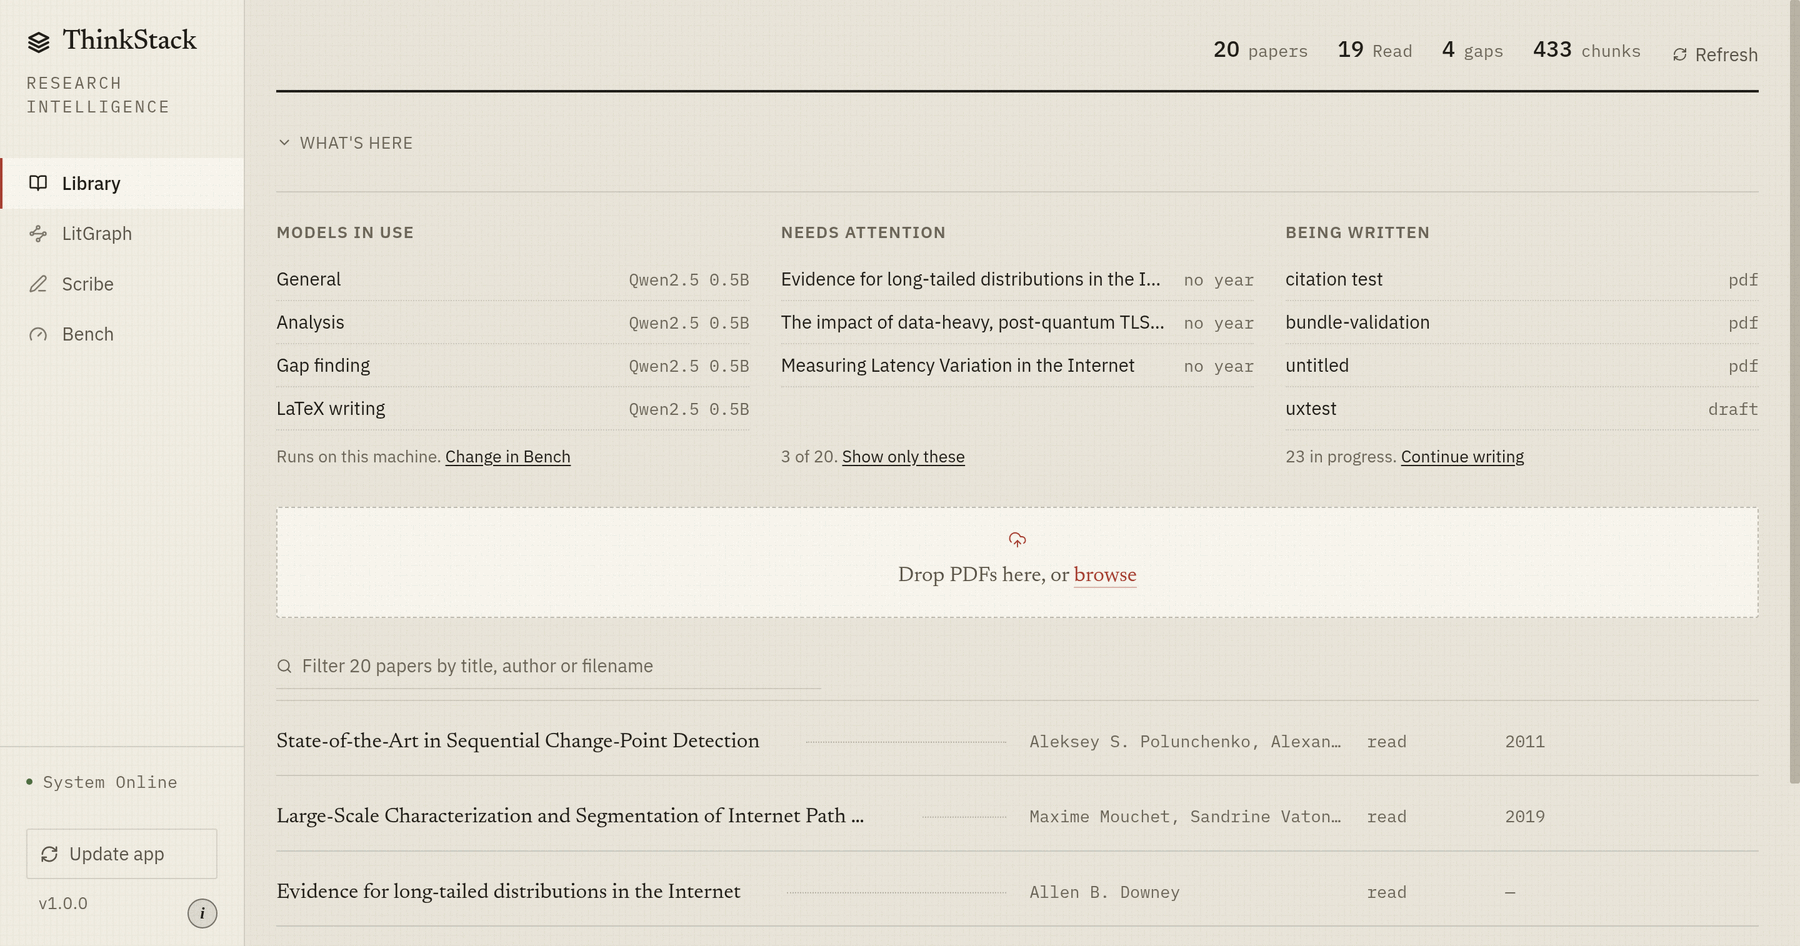
\includegraphics[width=\linewidth]{assets/screens/library.png}
\caption{Library. The folio above the rule counts the collection; the three
panels report which model serves which task, which papers are missing a field,
and which drafts are open. The shelf lists the papers themselves.}
\label{fig:library}
\end{figure}

\begin{figure}[H]
\centering
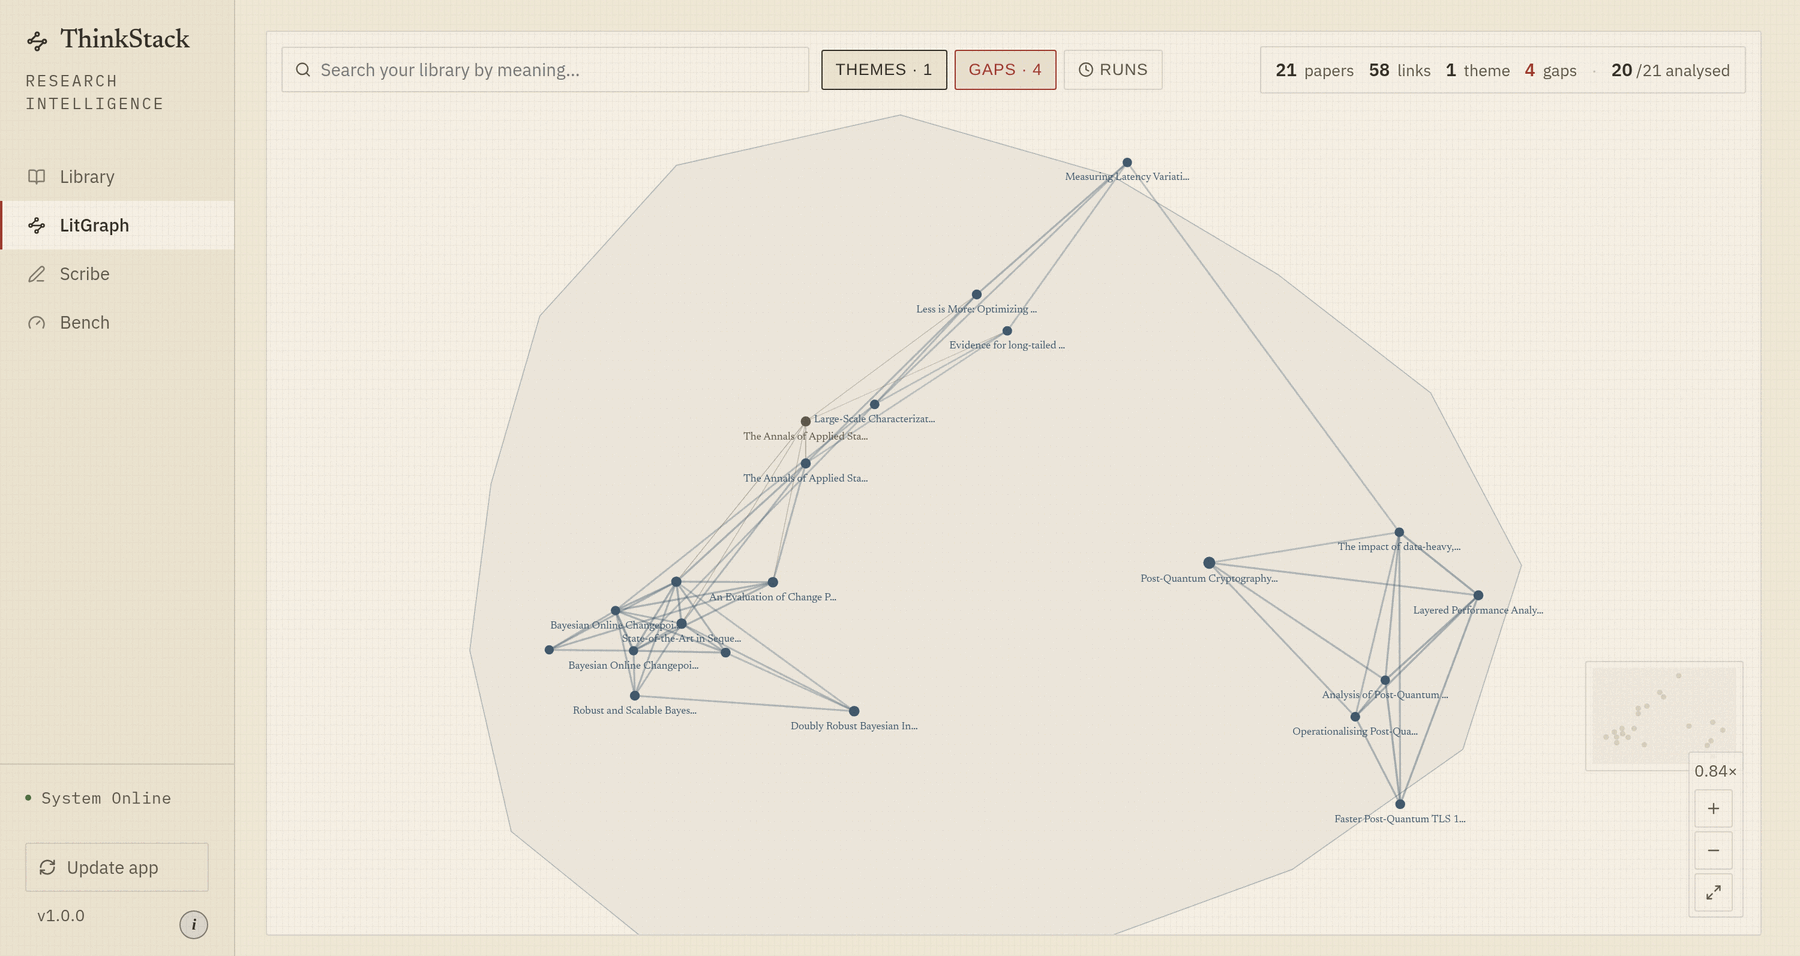
\includegraphics[width=\linewidth]{assets/screens/litgraph.png}
\caption{LitGraph. Papers are placed by semantic similarity, themes are drawn
as regions, and links show the strongest relations. Search, gap finding and the
encrypted vault are reached from this one view.}
\label{fig:litgraph}
\end{figure}

\begin{figure}[H]
\centering
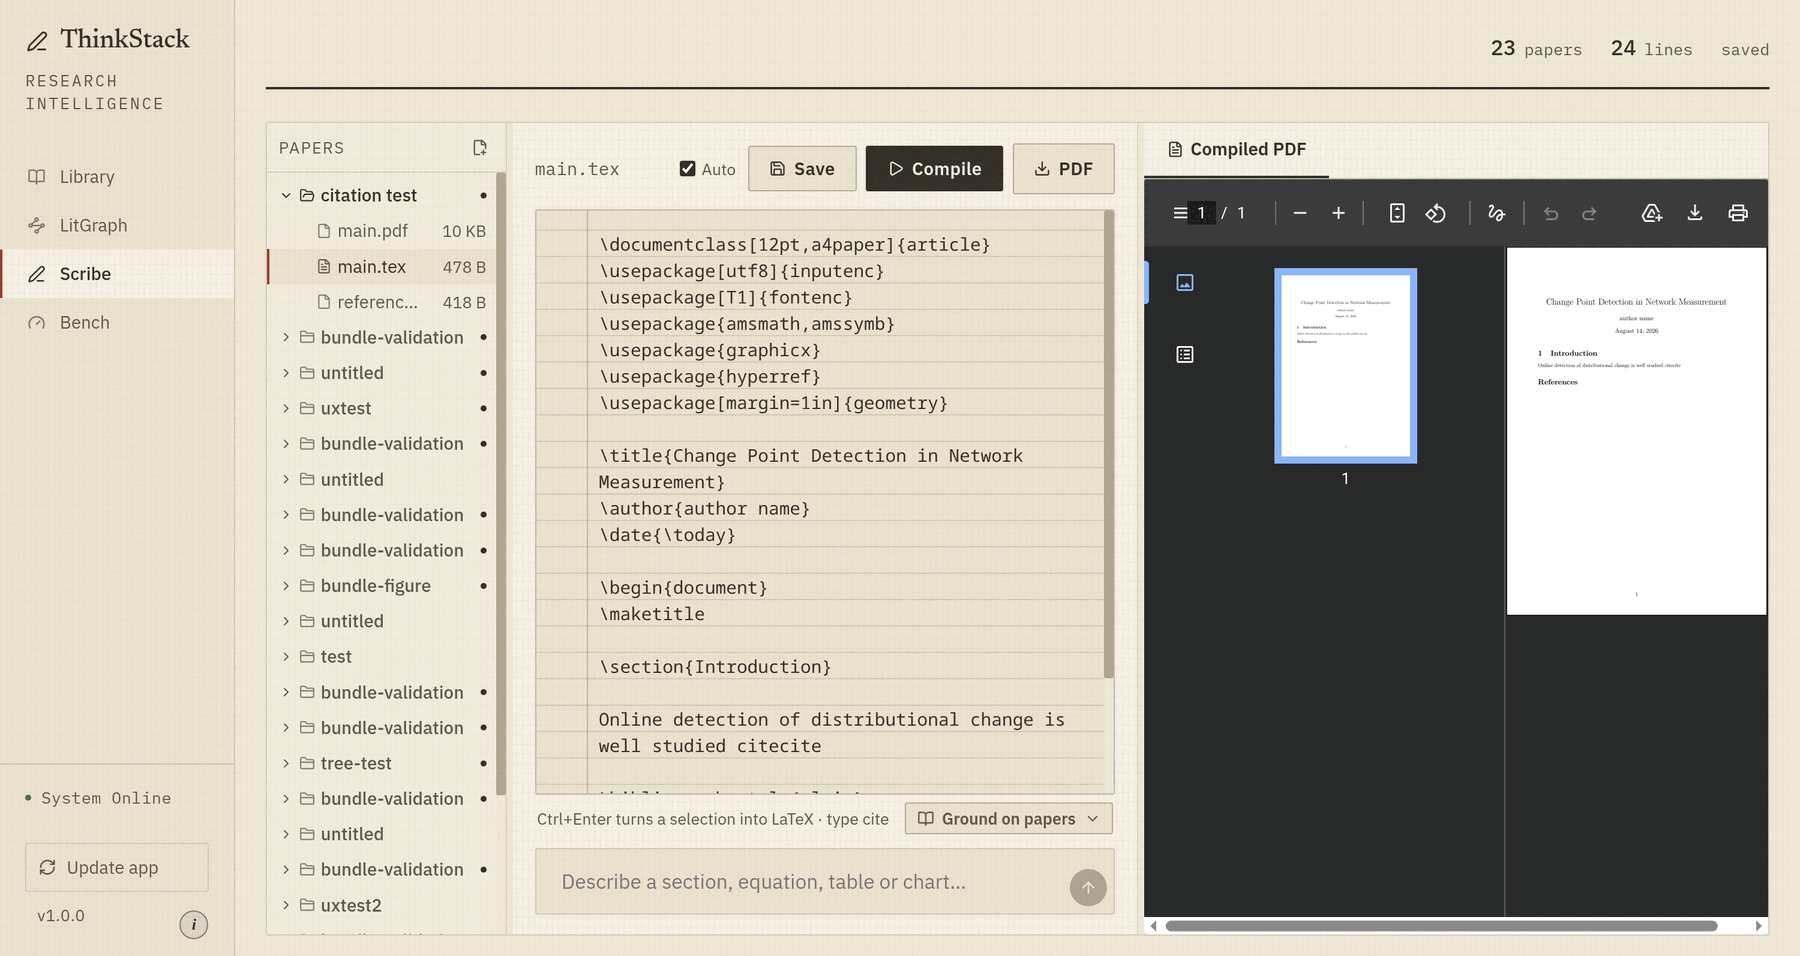
\includegraphics[width=\linewidth]{assets/screens/scribe.png}
\caption{Scribe. The project is a directory: the tree on the left, the source
in the middle, and the compiled PDF on the right, rebuilt a moment after typing
stops.}
\label{fig:scribe}
\end{figure}

\begin{figure}[H]
\centering
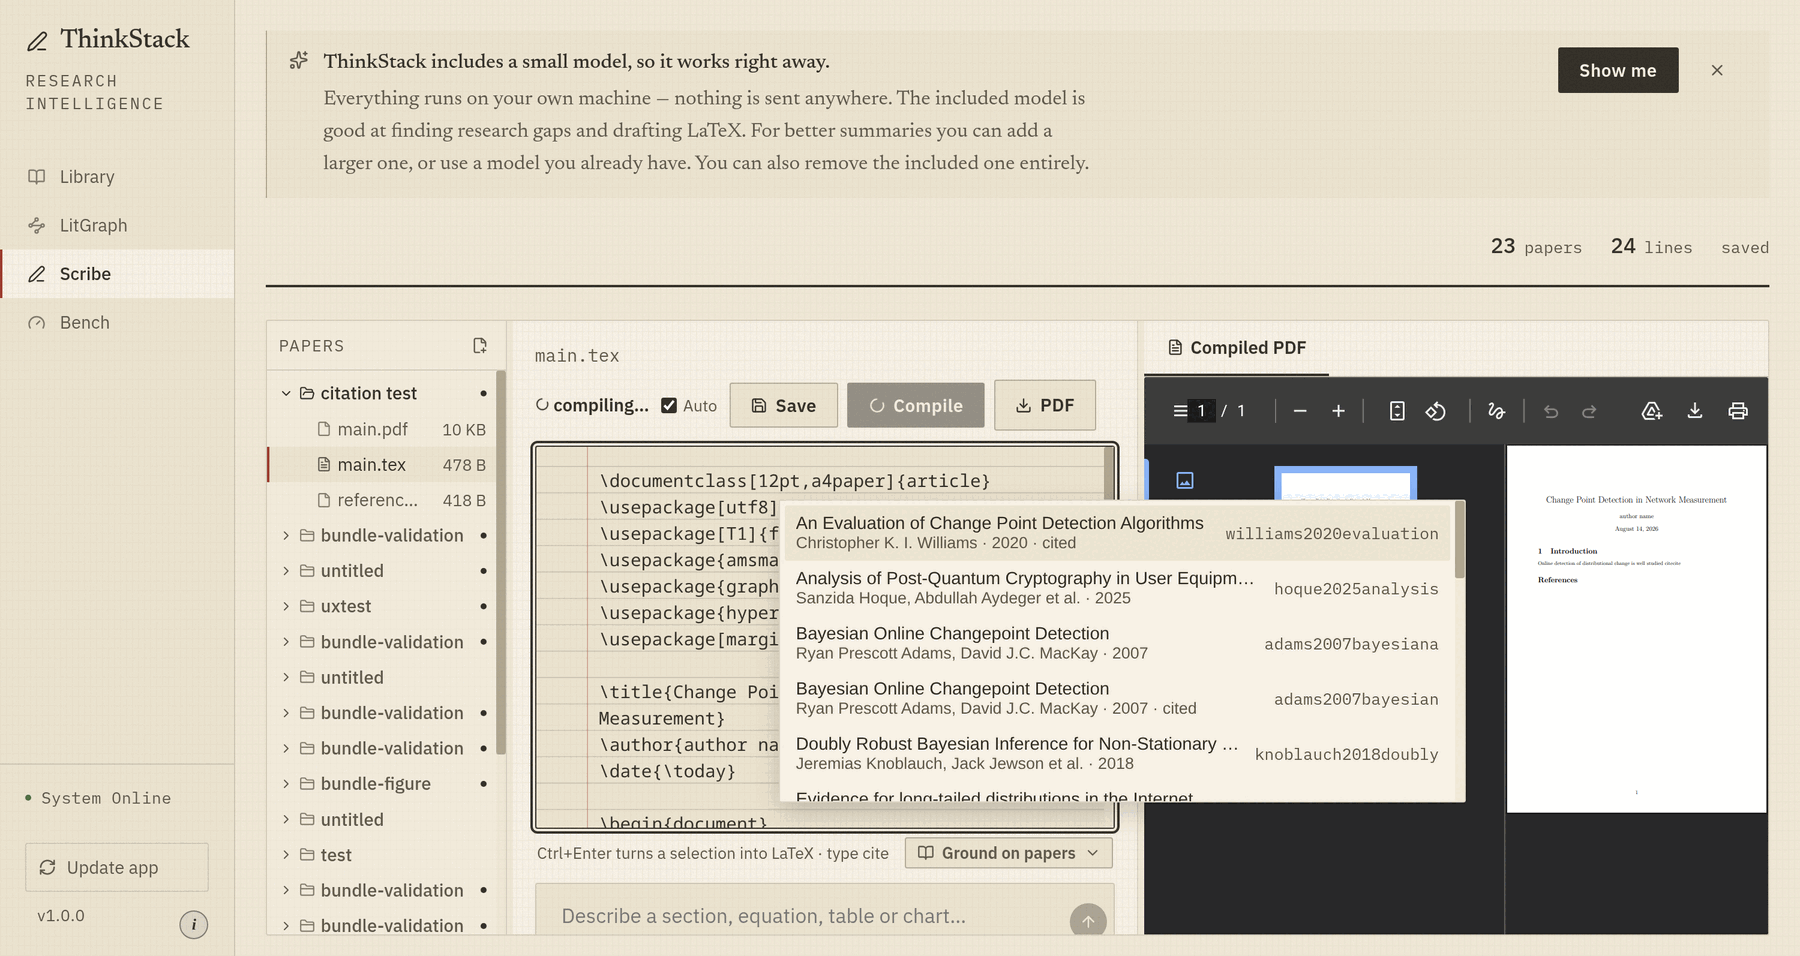
\includegraphics[width=\linewidth]{assets/screens/scribe-cite.png}
\caption{Citing from the editor. Typing the word \texttt{cite} opens the
library beneath the cursor, with the key each paper would be cited by shown at
the right and papers already in this project's bibliography marked. Enter
replaces the word with the citation command.}
\label{fig:cite}
\end{figure}

\begin{figure}[H]
\centering
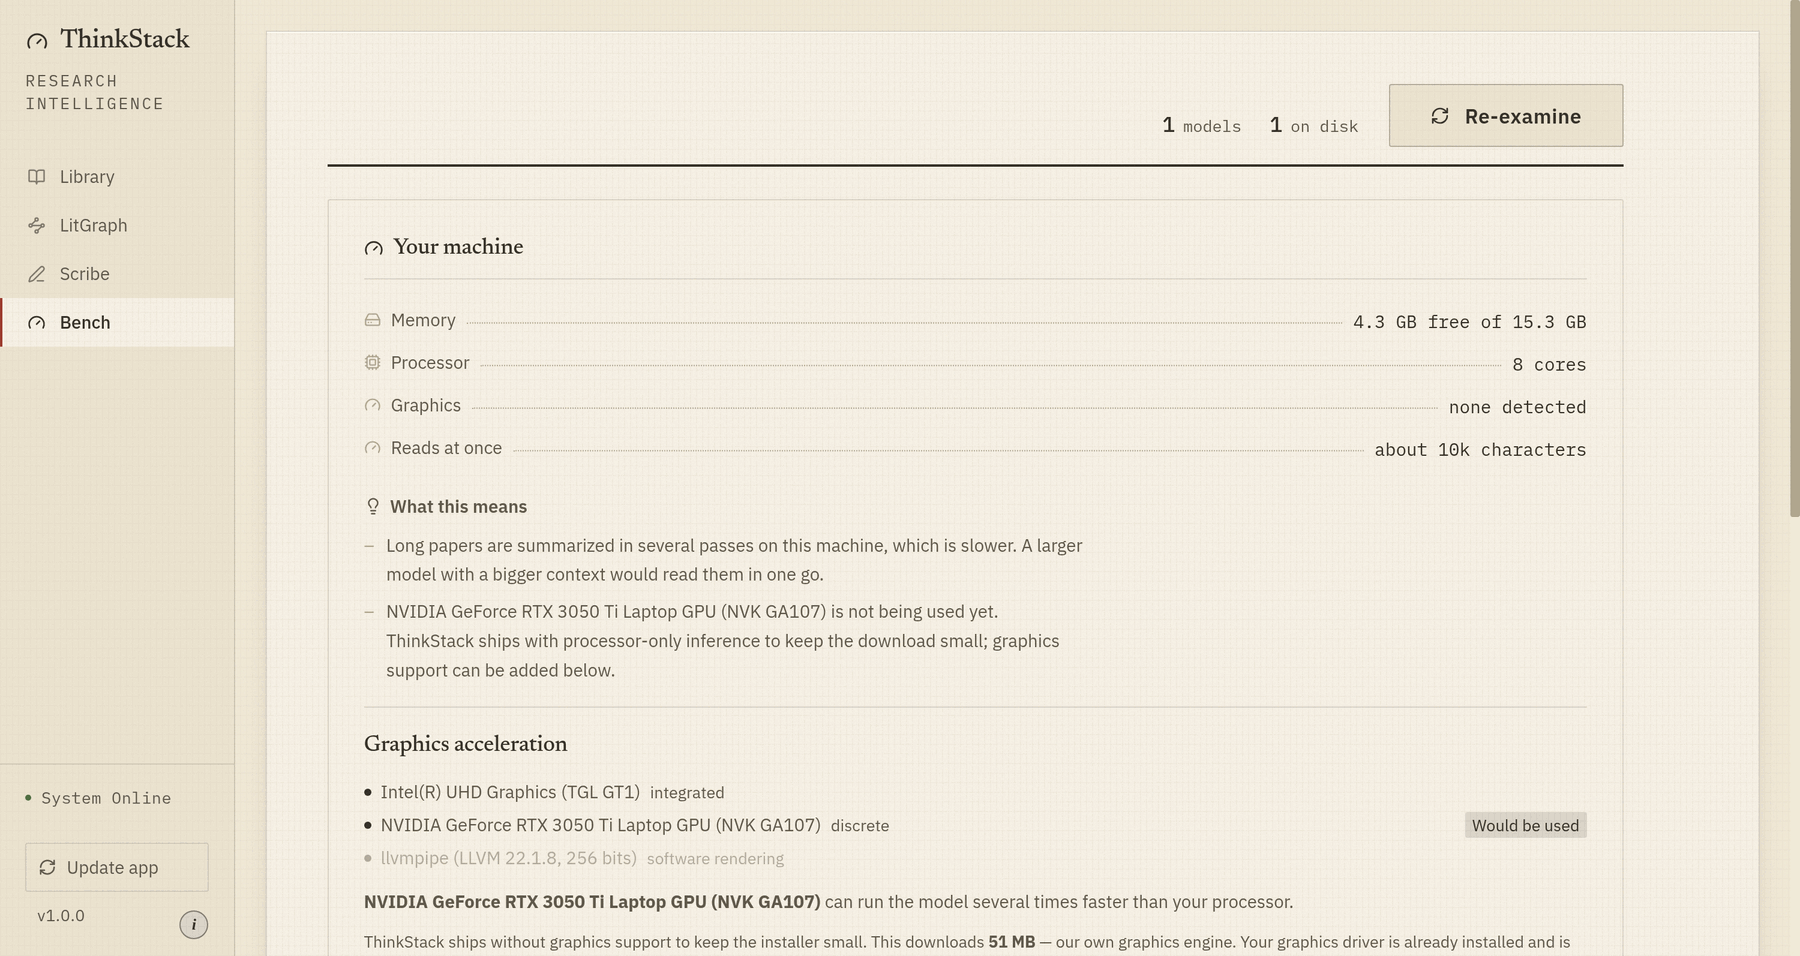
\includegraphics[width=\linewidth]{assets/screens/bench.png}
\caption{Bench. What the machine can run, measured rather than assumed,
including a graphics device that is present but not in use because the shipped
build is processor-only.}
\label{fig:bench}
\end{figure}

% ============================================================
\chapter{TESTING}
% ============================================================

\section{Testing Approaches}

Testing is in four layers, and the reason for the fourth is the interesting one.

\begin{longtable}{@{}p{0.24\linewidth}p{0.16\linewidth}p{0.54\linewidth}@{}}
\caption{Test layers}\label{tab:testlayers}\\
\toprule
\textbf{Layer} & \textbf{Count} & \textbf{What it establishes} \\
\midrule
\endfirsthead
\toprule
\textbf{Layer} & \textbf{Count} & \textbf{What it establishes} \\
\midrule
\endhead

Backend unit tests & 984 & Domain and infrastructure behaviour, run on every
  push and in CI. \\
Interface unit tests & 198 & Component and utility behaviour under jsdom. \\
Contract tests & 5 & That every route the interface calls is a route the
  backend defines: both sides parsed from source. \\
Packaged-application validation &: & That the \emph{installed} application
  starts and works, run against the built installer on each platform. \\
\bottomrule
\end{longtable}

The fourth layer exists because of a specific failure. Version 1.0.0 passed
every test and every build, was published, and did not start: the frozen backend
silently omitted the inference library's shared objects and the embedding
model's data, because neither package ships a hook for the freezer. A test suite
that runs from a source checkout cannot see that. \texttt{validate\_bundle.py}
now runs against the packaged application and checks outcomes rather than
statuses: for example, inspecting a compiled PDF for an image object rather
than trusting a ``compiled'' result, because a compile that silently drops the
figure also reports success.

\section{Test Cases}

Representative cases from each area; the full suite is in \texttt{tests/}.

\begin{longtable}{@{}p{0.07\linewidth}p{0.35\linewidth}p{0.34\linewidth}p{0.14\linewidth}@{}}
\caption{Representative test cases}\label{tab:cases}\\
\toprule
\textbf{ID} & \textbf{Case} & \textbf{Expected} & \textbf{Result} \\
\midrule
\endfirsthead
\toprule
\textbf{ID} & \textbf{Case} & \textbf{Expected} & \textbf{Result} \\
\midrule
\endhead

T-01 & Title is the largest horizontal text at the top of page 1 & Exact title
  returned & Pass \\
T-02 & Rotated archive stamp larger than the title & Stamp ignored & Pass \\
T-03 & Small-capitals title (two sizes, one baseline) & Whole title, no split
  & Pass \\
T-04 & Accent stored before its letter & Surname recomposed & Pass \\
T-05 & Affiliation row naming two employers, only one listed & Whole row
  rejected & Pass \\
T-06 & Phrase repeated in the author region & Treated as an address & Pass \\
T-07 & Year from an archive identifier vs. a stray four-digit number & Identifier
  wins & Pass \\
T-08 & Paper stating no year & Year left empty & Pass \\
T-09 & Plausible title, no authors & Model fallback invoked & Pass \\
T-10 & Model returns an empty field & Existing good value retained & Pass \\
T-11 & Correction propagates to every chunk & All chunks updated & Pass \\
T-12 & Correction with a blank title & Rejected, 400 & Pass \\
T-13 & Correction to an absent document & 404, nothing written & Pass \\
T-14 & Ingest continues when the analysis queue fails & Document retained
  & Pass \\
T-15 & PDF route for an encrypted document & Refused, 403 & Pass \\
T-16 & Filename escaping the project directory & Refused & Pass \\
T-17 & Sidebar collapse does not swallow the click that caused it & Click
  delivered & Pass \\
T-18 & Update prompt where the platform cannot ask & Not installed & Pass \\
T-19 & Every interface call resolves to a defined route & No orphans & Pass \\
T-20 & Version never decreases & Lower version refused & Pass \\
T-21 & An author list survives storage & Eight names read back as eight
  & Pass \\
T-22 & A key already in the bibliography is not recomputed & Same key returned
  & Pass \\
T-23 & Citing the same paper twice & One entry, same key & Pass \\
T-24 & An entry written by hand survives a citation & Retained & Pass \\
T-25 & Listing what can be cited writes nothing & No file created & Pass \\
T-26 & A citing document without a bibliography & Command supplied, references
  typeset & Pass \\
T-27 & Special characters in a title reach the bibliography & Escaped & Pass \\
T-28 & A JavaScript module is served as JavaScript & Never
  \texttt{text/plain} & Pass \\
T-29 & The same gap returned twice & One finding, evidence merged & Pass \\
T-30 & A selectable target on the map & 28\,px at every usable zoom & Pass \\
\bottomrule
\end{longtable}

\section{Test Reports}

\subsection{Metadata extraction, measured on unseen papers}

The development set was 18 papers chosen by the authors, on which the rebuilt
extractor was exactly correct on every title, author list and year. That figure
was then discarded as unsafe, because a measurement taken over material one has
selected oneself describes the selection rather than the method.

A second measurement was constructed in which neither the papers nor the
expected answers were chosen by the authors: 56 papers sampled across 15 arXiv
subject classifications through the public interface, scored against the
archive's own catalogue records.

\begin{longtable}{@{}p{0.34\linewidth}p{0.20\linewidth}p{0.20\linewidth}@{}}
\caption{Extraction accuracy, curated versus randomly sampled papers}\label{tab:extraction}\\
\toprule
\textbf{Field} & \textbf{Curated (18)} & \textbf{Random (56)} \\
\midrule
\endfirsthead
\toprule
\textbf{Field} & \textbf{Curated (18)} & \textbf{Random (56)} \\
\midrule
\endhead

Title exactly correct        & 100\%  & 92.9\% \\
Author list exactly correct  & 100\%  & 85.7\% \\
Year exactly correct         & 100\%  & 92.9\% \\
All three simultaneously     & 100\%  & 76.8\% \\
\bottomrule
\end{longtable}

The first random measurement was 62.5\% on all three fields. The entire
difference from the final figure was typesetting conventions that had not been
examined: one physics template spaces a centred author line widely enough to be
indistinguishable from column separation; another runs from the affiliations
into the abstract with no heading, so the search for authors continued into the
body; and a margin threshold introduced to discard an archive stamp was
discarding the first line of any centred title wide enough to begin left of it.

Of the 13 remaining failures, three are not extraction errors: the page reads
``M.~GRENDÁR'' and ``Audrey Quessadda-Vial'' where the archive record says
otherwise.

\subsection{Suite results}

\begin{longtable}{@{}p{0.34\linewidth}p{0.14\linewidth}p{0.14\linewidth}p{0.24\linewidth}@{}}
\caption{Suite results at the time of writing}\label{tab:suites}\\
\toprule
\textbf{Suite} & \textbf{Tests} & \textbf{Passing} & \textbf{Runtime} \\
\midrule
\endfirsthead
\toprule
\textbf{Suite} & \textbf{Tests} & \textbf{Passing} & \textbf{Runtime} \\
\midrule
\endhead

Backend (pytest)      & 1\,085 & 1\,084 & \textasciitilde14\,s \\
Interface (vitest)    & 222 & 222 & \textasciitilde5\,s \\
Contract              & 5   & 5   & $<$1\,s \\
Route reachability    & 16  & 16  & $<$2\,s \\
\bottomrule
\end{longtable}

Route reachability is distinct from the contract test and was added when the
interface was replaced. Parsing both sides as text proves the paths
\emph{match}; calling them against a running backend proves the handlers
\emph{run}.

% ============================================================
\chapter{CONCLUSION}
% ============================================================

\section{Design and Implementation Issues}

\subsection{A guard cannot test for the absence of a failure it never produces}

Three defects shared one shape, described in Section~\ref{sub:silence}, and it is the
single most transferable finding of the project. Each was a check written
against silence when the real failure was confident wrongness. The lesson is to
test for the shape of a right answer rather than for the absence of a wrong one.

\subsection{Constants standing in for measurements}

Two panes sized themselves as \texttt{calc(100vh - 11rem)}, with a comment
estimating the height of the page heading. Removing the heading made the
constant wrong, silently, and the correction had to be re-derived per screen.
Replacing it with a layout that takes the height it is given failed on the first
attempt, because the property used resolves against the nearest enclosing
flexible container and an unclassed wrapper sat between the two. The general
form: a guessed constant fails quietly, and replacing a mechanism requires
knowing what it sits inside.

\subsection{Measuring on material one has chosen}

The extractor scored 100\% on the authors' own test set and 62.5\% on a random
sample. Nothing about the development set was dishonest; it was drawn from a
single field, and a template is a convention of a field.

\subsection{Replacing a running interface costs double}

The interface was rebuilt as a parallel tree while the original kept shipping.
Every fix made during that period was made twice, and copying between the trees
was not available, because the replacement names its colour tokens the way the
original named its sizes. The mitigation, running both through the same CI
matrix, and parameterising the contract test over both, was necessary
precisely because the tree nobody is looking at is the one that rots.

\section{Advantages and Limitations}

\subsection{Advantages}

\begin{itemize}[leftmargin=*]
  \item No document, prompt or embedding leaves the machine, which makes the
        system usable on material that cannot be uploaded.
  \item No per-query cost and no account.
  \item Fully functional offline, including typesetting.
  \item Metadata accurate enough to label a paper and populate a citation:
        92.9\% of titles on unseen papers.
  \item Sized to the machine, so a consumer laptop is the target rather than the
        degraded case.
  \item Distributed and verified as installers on three platforms, with the
        packaged application itself under test.
\end{itemize}

\subsection{Limitations}

\begin{itemize}[leftmargin=*]
  \item \textbf{Model capability.} A 0.5B model produces malformed structured
        output on the harder tasks; those route to a 1.5B when one is present
        and degrade when it is not.
  \item \textbf{Scanned documents.} No text layer means nothing to read. OCR is
        not shipped.
  \item \textbf{Extraction tail.} Mathematics inside a title, publisher cover
        pages, and submissions with no identifier still defeat the rules.
  \item \textbf{Retrieval quality.} Measured on one query, the top-ranked
        passage scored 0.212 where a good match on this embedding model is
        0.45--0.70, and a cover page outranked the passage containing the
        answer. The probable cause is chunk size diluting the signal. This is
        unresolved and is stated rather than omitted.
  \item \textbf{Citations.} Entries can be generated from extracted metadata but
        will be incomplete: venue, volume and pages are not recoverable from
        page one.
  \item \textbf{No collaboration or synchronisation}, which follows from the
        premise.
\end{itemize}

\section{Future Scope}

\begin{enumerate}[leftmargin=*]
  \item \textbf{A layout classifier for metadata.} The remaining extraction
        failures are a long tail of typesetting conventions, and each currently
        costs another rule. The established answer is a small classifier over
        the same features the rules already read: font size, position,
        capitalisation, row order, which is what GROBID does with a
        conditional random field at roughly 90\% F1. The research interest is
        not the classifier but the constraint: GROBID needs a JVM and a model
        server, and the neural alternative needs a GPU. \emph{Nobody optimises
        this task for a CPU-only machine with no network}, which is the
        constraint this application is built under, and measuring how close a
        fixed budget gets to those ceilings is publishable either way.
  \item \textbf{Remembering corrections.} When a user fixes a wrong title, store
        the page's layout fingerprint against the correction. Papers arrive in
        clusters from the same venues, so one correction pays for itself
        repeatedly. This is adaptation without gradients: inspectable,
        reversible, and free of the forgetting that on-device fine-tuning of a
        shared model would risk.
  \item \textbf{Citations in Scribe.} The application has already read the
        paper, so the entry a hosted editor makes the author fetch by hand is
        already in the library. The compiler already runs BibTeX, so this needs
        no compiler change.
  \item \textbf{Source-to-output synchronisation.} The compiler already emits a
        SyncTeX map on every build and nothing reads it. Click-through in both
        directions is available for the cost of parsing a file already on disk.
  \item \textbf{Fine-tuned task models.} A model trained on instruction-to-markup
        pairs, for which data is already collected passively during use.
  \item \textbf{Retrieval quality.} The 0.212 result deserves its own
        investigation with a proper query set.
\end{enumerate}

% ============================================================
\chapter*{REFERENCES}
\addcontentsline{toc}{chapter}{References}
% ============================================================

\begin{enumerate}[leftmargin=*]
  \item Vaswani, A., Shazeer, N., Parmar, N., \emph{et al.} ``Attention Is All
        You Need.'' \emph{Advances in Neural Information Processing Systems},
        2017. arXiv:1706.03762.
  \item Reimers, N. and Gurevych, I. ``Sentence-BERT: Sentence Embeddings using
        Siamese BERT-Networks.'' \emph{EMNLP}, 2019. arXiv:1908.10084.
  \item Lewis, P., Perez, E., Piktus, A., \emph{et al.} ``Retrieval-Augmented
        Generation for Knowledge-Intensive NLP Tasks.'' \emph{NeurIPS}, 2020.
        arXiv:2005.11401.
  \item Lopez, P. ``GROBID: Combining Automatic Bibliographic Data Recognition
        and Terminology Recognition.'' \emph{ECDL}, 2009.
  \item Blecher, L., Cucurull, G., Scialom, T. and Stojnic, R. ``Nougat: Neural
        Optical Understanding for Academic Documents.'' 2023.
        arXiv:2308.13418.
  \item Yang, A., Yang, B., Hui, B., \emph{et al.} ``Qwen2.5 Technical Report.''
        2024. arXiv:2412.15115.
  \item Gerganov, G. \emph{llama.cpp: LLM inference in C/C++.} 2023.
        \url{https://github.com/ggerganov/llama.cpp}
  \item Biggs, N. \emph{Tectonic: A modernized, complete, self-contained \TeX{}
        engine.} \url{https://tectonic-typesetting.github.io}
  \item Tauri Contributors. \emph{Tauri: Build smaller, faster, more secure
        desktop applications.} \url{https://tauri.app}
  \item Ramírez, S. \emph{FastAPI.} \url{https://fastapi.tiangolo.com}
  \item Biham, E. and Dunkelman, O. ``Argon2: the memory-hard function for
        password hashing.'' \emph{IETF RFC 9106}, 2021.
  \item Adams, R. P. and MacKay, D. J. C. ``Bayesian Online Changepoint
        Detection.'' 2007. arXiv:0710.3742.
\end{enumerate}

\end{document}
